\documentclass[11pt]{article}
\usepackage[margin=0.85in]{geometry}
\usepackage{amsmath,amssymb}
\usepackage{booktabs}
\usepackage{graphicx}
\usepackage{xcolor}
\usepackage{titlesec}
\usepackage{enumitem}
\usepackage[colorlinks=true,linkcolor=blue!55!black]{hyperref}

\definecolor{ink}{HTML}{1A1A1A}
\definecolor{muted}{HTML}{5C5A54}
\titleformat{\section}{\normalsize\bfseries\color{ink}}{\thesection.}{0.5em}{}
\setlength{\parskip}{4pt}
\setlength{\parindent}{0pt}

\newcommand{\JV}{\mathrm{JV}}
\newcommand{\TPV}{\mathrm{TPV}}
\newcommand{\code}[1]{\texttt{\small #1}}

\begin{document}
\thispagestyle{empty}

{\LARGE\bfseries Bitcoin jump clustering and the variance risk premium}\\[4pt]
{\large\color{muted} Does a running jump cluster tell you the premium is about to compress?}\\[8pt]
{\color{muted}\small 1{,}838{,}880 one-minute bars, Jan 2023 to Jun 2026 \quad$\cdot$\quad
Deribit DVOL \quad$\cdot$\quad code and derivations in the repository}

\vspace{6pt}\hrule\vspace{8pt}

Bitcoin's price jumps arrive in bunches rather than evenly, which is easy enough
to see by eye. What I wanted to know is whether that buys you anything: if a
bunch is happening right now, does it say the options market is about to get
cheaper? The trouble is that ``how agitated the jump process currently is'' is
not something you observe. So most of the work here is building a model that can
estimate it, checking that the model actually works, and only then asking the
question I started with.

\section{What I found}

\subsection*{Jumps cluster, and the standard model has no room for it}

The usual jump-diffusion setup has jumps arriving at a constant rate. That
carries a consequence you can check directly: jump energy on separate days is
independent, so the autocovariance of daily jump variance is zero at every lag,
for any parameter values whatsoever. There is nothing to tune.

It is not zero.

\begin{center}\small
\begin{tabular}{lcc}
\toprule
test & constant-intensity model says & data\\
\midrule
Jump clustering, $\mathrm{Cov}(\JV_t,\JV_{t-k})$, joint over 10 lags & $0$ & $t = 3.05$\\
Diffusive variance leading future jumps, joint over 5 lags & $0$ & $t = 2.78$\\
Lag-1 jump clustering on its own & $0$ & $t = 3.74$\\
\bottomrule
\end{tabular}
\end{center}

\begin{center}
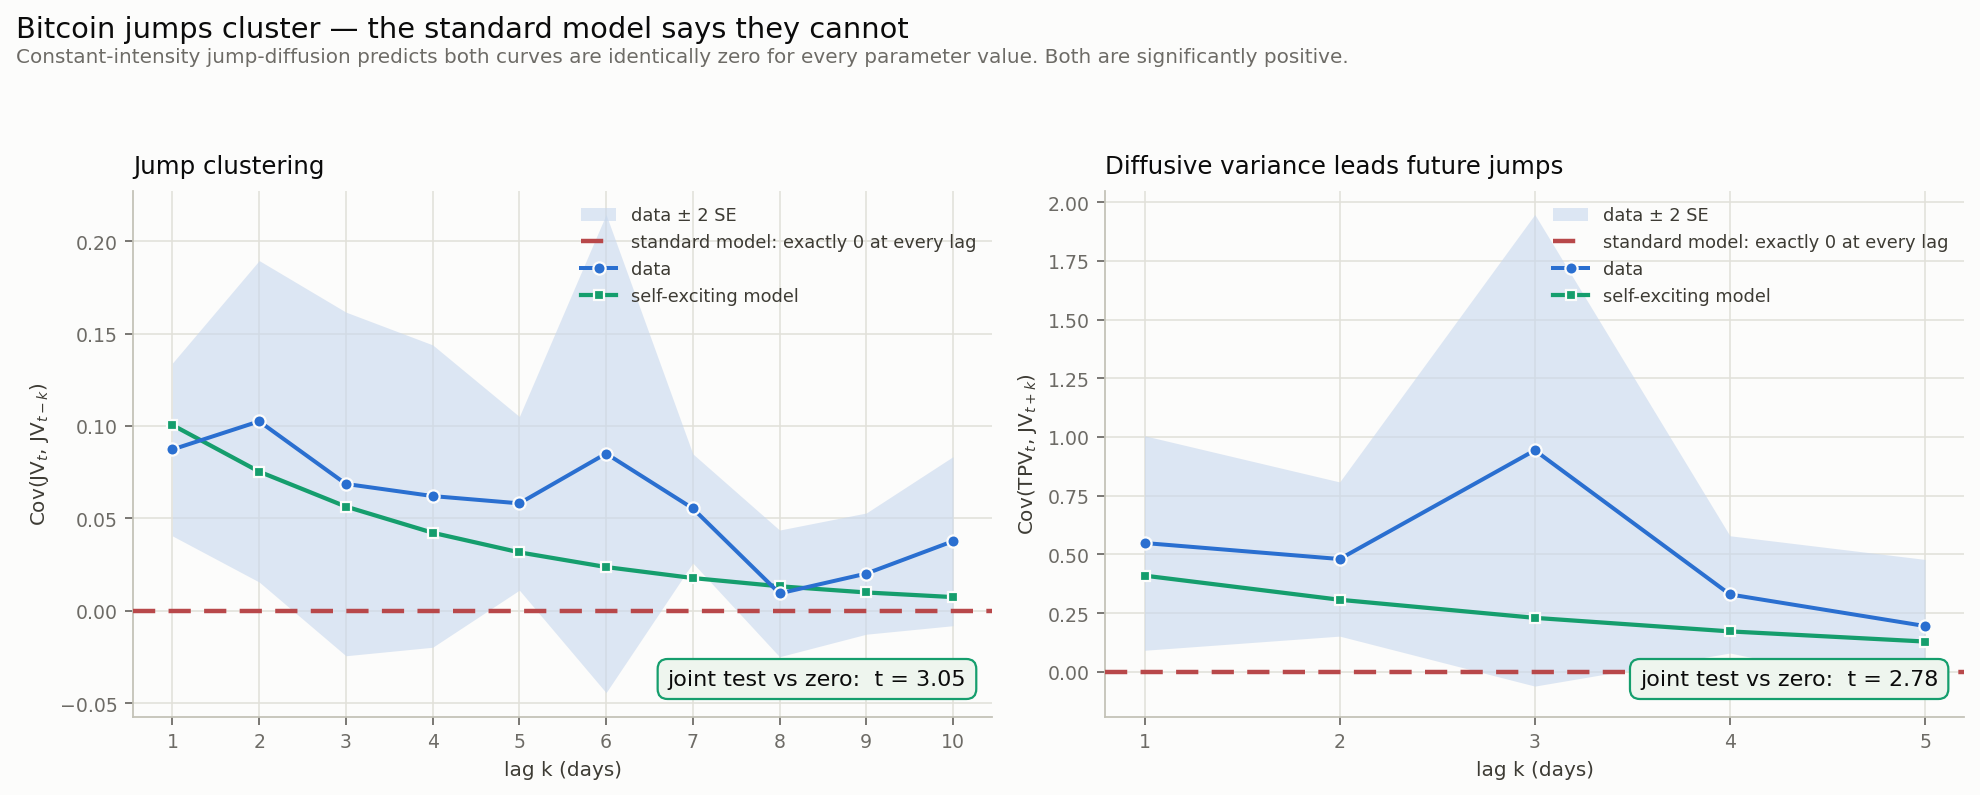
\includegraphics[width=\textwidth]{FIG1_finding.png}
\end{center}

\subsection*{Letting jumps excite themselves fixes it}

The repair is to make the arrival rate depend on the jump-variance state,
$\lambda(t)=\lambda_0+\lambda_1 V^j(t^-)$, so a jump raises the odds of the next
one. Both curves above come back. Fitting by GMM on 40 moments, 2 of the 40 miss
by more than two standard errors, which is roughly what noise alone gives you,
and the misses are scattered instead of piling up in one block.

The estimates put about 24\% of jumps down as aftershocks of earlier jumps. A
single shock fades with a 1.8 day half-life, but a whole cluster takes 2.4 days,
which is the point of the extension: the cascade outlives the shock that started
it.

\subsection*{The premium is large}

Implied variance sits around 20\% above what the model expects physically, on
65\% of days, and about 25\% above what actually gets realised. It mean-reverts
with a half-life of roughly two weeks.

\subsection*{The model still decays too fast}

On held-out crash events, variance stays elevated about 9.5 days. My model says
2.4. A separate over-identification check disagrees with the model in the same
direction (by a factor of 6.3), so I think something slow is genuinely missing,
most likely a third variance factor. The self-exciting term moves things the
right way but not nearly far enough.

\section{Checking the machinery before I used it}

This is where most of the time went. The 40 moments are closed-form expressions the
model implies, and if I get any one of them wrong then everything downstream is
quietly wrong with it, in a way that no amount of staring at the output would
reveal.

So before running anything on real data I wrote an exact simulator: Ogata
thinning for the self-exciting jumps, the noncentral $\chi^2$ transition for the
CIR factor, and analytic integrals within each day, so there is no discretisation
error anywhere to hide behind. Then I generated 50{,}000 days from each of six
known parameter sets and checked every formula against what the simulation
actually produced.

\begin{center}
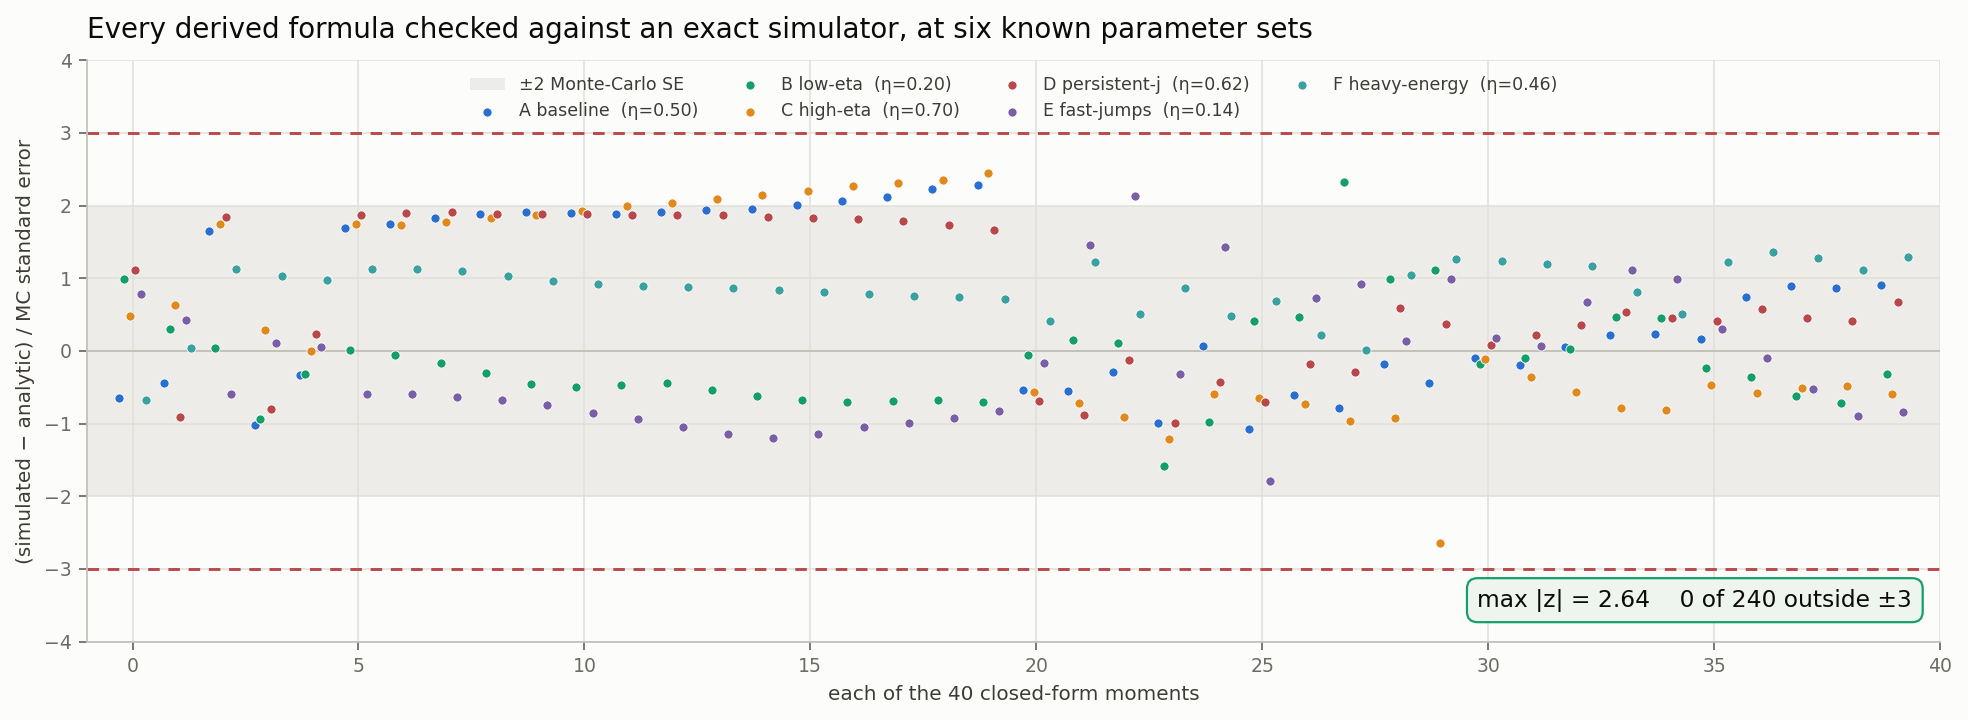
\includegraphics[width=\textwidth]{FIG2_verification.png}
\end{center}

Everything landed inside Monte Carlo error, with a maximum $|z|$ of 2.64 and none
of the 240 outside $\pm3$. GMM recovered the true parameters, and the bootstrap
intervals covered at 0.86 to 0.98 against a nominal 0.95.

Doing this caught four real bugs:

\begin{itemize}[leftmargin=1.4em]
\item My tripower variation used exponent $4/3$, which estimates quarticity, when
variance needs $2/3$. The ``jump variance'' series was effectively total
variance. I found it by cross-checking against MedRV, a second jump-robust
estimator, which now agrees at $\rho = 0.996$.
\item The block bootstrap was resampling the raw series and recomputing lag
products on the result, which splices unrelated days together at every block
join. Coverage for one parameter came out at 0.00. Resampling the moment
contributions instead put it back to 0.93.
\item The GMM weighting matrix was shrinking toward a scaled identity, which
ignores that moment variances here span five orders of magnitude, so the
jump-clustering moments got almost no weight. This had inverted the persistence
estimate, 3.43 against the correct 0.29, and I only noticed from the fit
residuals.
\item One of my two over-identification tests turned out to be an algebraic
tautology. It holds for any parameter values at all, so it tested nothing, and I
had already written it up as a pass. The giveaway was that it came out exactly
zero with exactly zero variance in every bootstrap draw, and real quantities
wobble.
\end{itemize}

\newpage

\section{The question I started with, and the answer}

Sorting days by how rich the premium is and how hot the jump state is gives a
clean pattern in sample. Holding the premium rich, a hot jump state compresses it
roughly 20 times harder over the next ten days than a quiet one does, and raises
the odds of a large compression by about 2.1 times.

\begin{center}
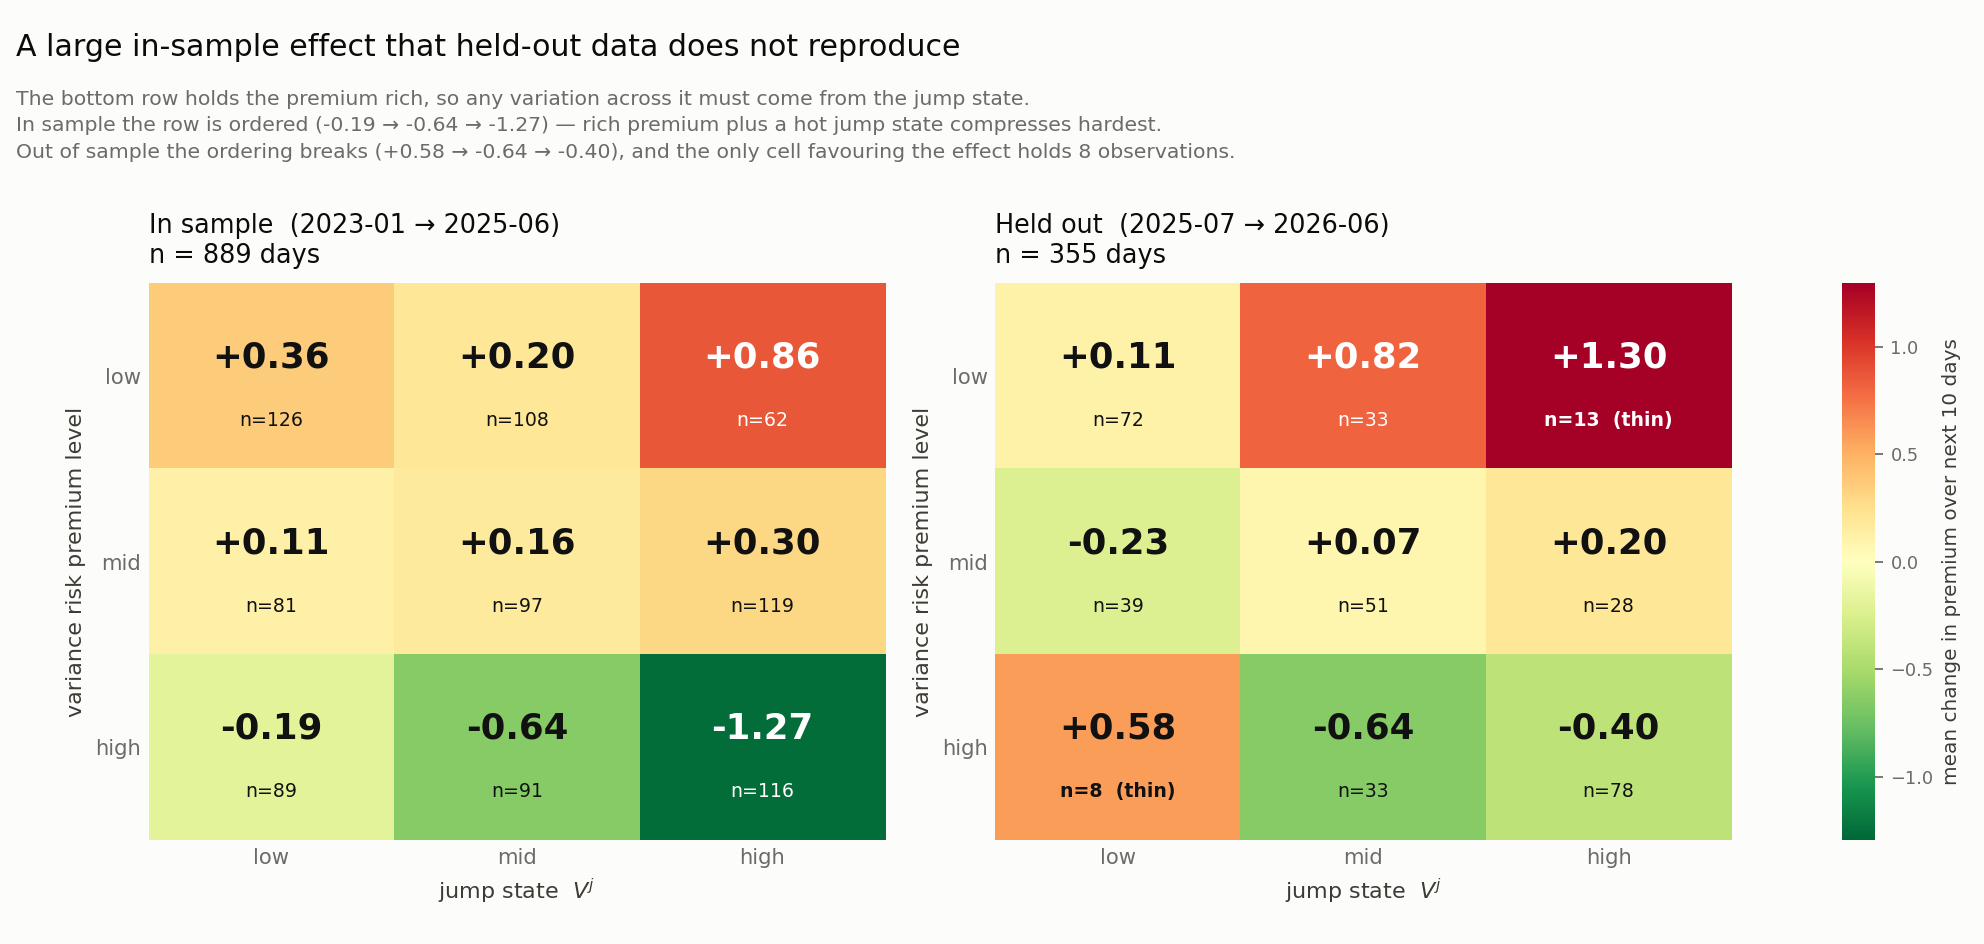
\includegraphics[width=\textwidth]{FIG3_honest_limit.png}
\end{center}

It does not hold up out of sample. On the held-out year the ordering breaks, and
the one cell that would support the effect has 8 observations in it. With
something like 35 independent ten-day windows the holdout cannot really settle
the question either way, but it certainly did not confirm anything.

Three other results looked good and did not survive being tested properly:

\begin{itemize}[leftmargin=1.4em]
\item The premium appeared to predict variance-selling returns at $t = 5.7$. But
the signal and the payoff both contain the implied-variance leg, correlated at
0.97, and controlling for it leaves $t = 0.99$.
\item The continuous-variance state appeared to predict premium changes at
$t = 2.5$. But the model's forecast is constructed out of that state, so the
relationship is mechanical, $t = 8.5$ through that channel alone. Against pure
market data it is $t = 0.10$.
\item The structural forecast does not beat a three-term HAR regression,
$R^2$ of 0.117 against 0.113.
\end{itemize}

I would rather write all of this down than quietly keep whichever version looked
best.

\section{How it works}

Total variance comes from two latent factors: a persistent Brownian-driven CIR
component, and a jump-driven component whose arrival intensity is affine in its
own level. Affinity is what matters, because it keeps all 40 unconditional
moments in closed form. Those are the means, variances, autocovariances and
two-sided cross-covariances of daily tripower variation and jump variance, and I
match them to sample moments by GMM using an analytic $40\times9$ Jacobian,
regularised weighting, and a moving-block bootstrap for intervals.

Parameters come from 2023-01 to 2025-06 only. Everything from 2025-07 onward,
which includes the October 2025 crash, is held out and never touched during
estimation.

\section{What I would do next}

The persistence gap, 9.5 days observed against 2.4 predicted, and the
factor-of-6.3 over-identification gap both point at the same missing piece, so a
third and slower variance factor is the obvious thing to try. The compression
result needs more than one year of held-out data before it means anything either
way. At this point the sample size is the constraint, not the method.

\vspace{8pt}\hrule\vspace{6pt}
{\small\color{muted}
Everything reproduces with \code{python run\_all.py}. The derivations are in
\code{docs/affine\_intensity\_theory.pdf}.}

\end{document}
